\section{Sensibility Testbed Design}\label{sec-design}

This section describes the design of the Sensibility Testbed. 
%On one hand, Sensibility Testbed manages how device owners make their
%devices accessible to the research community. On the other hand,
%it offers technical resources to researchers that allow them to
%securely collect data from remote mobile devices. 
We start with
<<<<<<< HEAD
an overview of the principles behind the design of the testbed infrastructure (Section~\ref{sec-overview}), 
followed by a detailed description of each testbed component 
(Section~\ref{sec-component}). Lastly, we describe the testbed in operation.
 (Section~\ref{sec-ops}).
=======
an overview of the testbed infrastructure (Section~\ref{sec-overview}), 
and a description of each testbed component 
(Section~\ref{sec-component}), then finally describe the testbed in 
operation (Section~\ref{sec-ops}).
>>>>>>> yyzhuang/master


\subsection{Overview: Design Principles}\label{sec-overview}

%\subsubsection{Interacting Parties}\label{sec-parties}
The operation of Sensibility Testbed  involves three types of interacting
parties, as shown in Figure~\ref{fig-arch}: mobile \textit{devices} 
owned by ordinary people, with our app installed; a 
\textit{clearinghouse} server that discovers and configures
participating devices; and \textit{experimenters} who want to run
<<<<<<< HEAD
experiments on mobile devices. The interaction between these three components, which is illustrated in Figure~\ref{fig-arch}. is designed to support three fundamental design principles.
%\subsubsection{Testbed Architecture}

\textbf{Shared access to device resources.} 
Since hardware resources are limited on mobile devices, it is 
not possible to dedicate an entire device to an experiment. Therefore, 
Sensibility Testbed allows several experiments to share one device. It uses a sandbox to isolate one researcher's code from 
 another, through a technique called performance isolation. The sandbox 
also prevents experiment code from inadvertently harming the device
via security isolation. Other software within the device allows
it to communicate with the rest of the testbed. Together, they form the
\textit{device software} (Section~\ref{sec-repy}, though only the 
sandbox is shown in Figure~\ref{fig-arch}).

\textbf{A centralized way of allocating devices and mediating data access.}
Sensibility Testbed is designed to provide both enhanced security and more efficient management of experimental set-up, so another principle kept in mind for the design was a central component that could serve as a a trusted intermediary for acquiring and managing device resources. Both tasks are delegated to  a server called \textit{clearinghouse}~\cite{ch}. The clearinghouse allows researchers to 
register accounts for each experiment, and share access to a common 
pool of devices, freeing them from the need to individually recruit participants. 
The clearinghouse can also allocate resources and mediate 
data access according to policies defined by a researcher's IRB. The 
clearinghouse thus facilitates device sharing and policy enforcement 
(Section~\ref{sec-ch}).

\textbf{Local support for remote experimentation.} 
The last design principle was to allow researchers to manage their experiments on remote devices from a local machine, as is offered by other testbeds~\cite{hibler2008large, peterson2006experiences}. Sensibility 
Testbed addresses this need by using a tool called \textit{experiment manager). The experiment manager and provides access to 
=======
experiments on mobile devices. Sensibility Testbed provides 
a set of software components on each of these interacting
parties.

%\subsubsection{Testbed Architecture}

\textbf{Shared access to device resources.} 
Since the hardware resources are limited on mobile devices, it is 
not possible to dedicate an entire device to an experiment. Therefore, 
Sensibility Testbed allows sharing of a device among several 
experiments. It uses a sandbox to isolate researchers' code from 
one another through its performance isolation technique. The sandbox 
also prevents experiment code from inadvertently harming the device
via security isolation. Additionally, there is other software that allows
the device to communicate with the rest of the testbed. They form the
\textit{device software} (Section~\ref{sec-repy}, though only the 
sandbox is shown in Figure~\ref{fig-arch}).

\textbf{Allocating device resources.}
In order for researchers to gain access to devices, there needs to be a 
trusted intermediary for acquiring and managing device resources.
Sensibility Testbed uses a server called \textit{clearinghouse}~\cite{ch} to allow researchers to 
register accounts for each experiment, and share access to a common 
pool of devices. Without a clearinghouse, each researcher would 
need to individually recruit devices to participate in their experiment. 
The clearinghouse can also allocate resources and mediate 
data access according to policies defined by a researcher's IRB. It 
achieves this by enforcing policies at the remote sandboxes. The 
clearinghouse thus facilitates device sharing and policy enforcement 
(Section~\ref{sec-ch}).

\textbf{Supporting remote experimentation.} 
In a distributed testbed a researcher needs to manage experiments 
on remote devices directly from a local machine, like in many other 
testbeds~\cite{hibler2008large, peterson2006experiences}. Sensibility 
Testbed uses a tool called \textit{experiment manager} so that a 
researcher can control his experiments remotely. Such a tool 
executes on a researcher's local computer, and provides access to 
>>>>>>> yyzhuang/master
hardware resources on mobile devices using the researcher's testbed 
credentials (assigned by the clearinghouse). This tool will be introduced
in Section~\ref{sec-emt}.

\begin{figure}
\center{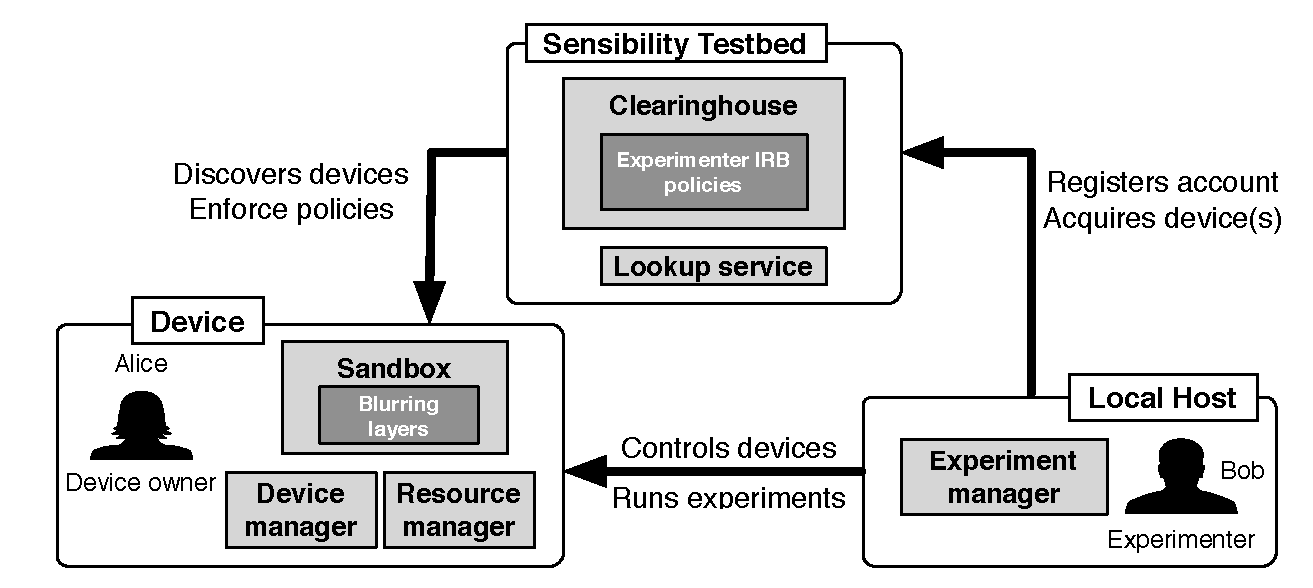
\includegraphics[width=\columnwidth]{figs/arch.pdf}}
%\vspace*{-20pt}
\caption{\small Sensibility Testbed architecture. \label{fig-arch}}
\end{figure}

<<<<<<< HEAD
=======

\smallskip
The following sections describe the three components in more detail, and 
addresses how these parties interact to enable safe experimentation on 
mobile devices. 
>>>>>>> yyzhuang/master

\smallskip
The following sections describe the three components in more detail
%\subsubsection{Enforcing IRB Approved Policies}


\subsection{Testbed Architecture}\label{sec-component}

<<<<<<< HEAD
As introduced above, the Sensibility Testbed architecture includes three main components that are critical to its operation. In this section, we discuss each of these components in greater detail, describing their functions and introducing several key techniques that make the testbed's enhanced security possible. The security aspects mentioned here and in 3.2.2 and 3.2.3 will be discussed in much greater detail in Section 4.
=======
The components of the Sensibility Testbed are shown in Figure~\ref{fig-arch}.
Each is critical to the operation of the testbed. 
In this section, we describe the function of each component.
>>>>>>> yyzhuang/master

\subsubsection{Device Software}\label{sec-repy}

%In Sensibility Testbed, all experiments execute in a secure 
%sandbox on the end devices.
%Experimenters' code executes in a sandbox that isolates the 
%experiment code from the device host system. 
<<<<<<< HEAD
The device software of Sensibility Testbed is the only one of the three components that the device users will interact with directly. It is divided into three parts: a secure sandbox called Repy (Restricted Python)\footnote{\scriptsize, a device manager that allows the owner to control what experiments can be run on his device, and a resource manager that facilitates interaction between experimenter's code and the sandbox received on the end-users mobile device.
The Repy sandbox is the most significant element in the device software. This security-reviewed sandbox~\cite{cappos2010retaining} used successfully for more than six years in our 
prior work, the Seattle testbed~\cite{seattle}, mitigates the impact of bugs in experimenter code by providing security isolation by physical separation of test code, and performance isolation by interposition on system calls. 
=======
The device software in Sensibility Testbed is divided into three parts. 
The most important one is a sandbox called Repy (Restricted 
Python)\footnote{\scriptsize This is the 
same security-reviewed sandbox~\cite{cappos2010retaining} used in
our prior work, the Seattle testbed~\cite{seattle}. This sandbox
mitigates the impact of bugs in experimenter code.}, which 
provides security isolation and performance isolation on mobile devices.
>>>>>>> yyzhuang/master
%Instead of developing full-fledged Android apps, all 
%experiments in Sensibility Testbed are written in a language
%similar to Python, and run in a secure %Python-based
Researchers use a Python-like programming interface~\cite{repyv2}
to write experiment code, upload the code and execute it in the
sandbox on remote devices. The programming interface includes functions for networking, 
file system access, threading, locking, logging, and so on. To access sensors, 
the sandbox also has a set of sensor functions~\cite{sensors}. 
%Details about implementing the Repy sandbox for mobile 
%devices are described in Section~\ref{sec-repy-ext}.
%
%However, the current Repy sandbox does not include calls to access sensors. 
%%To obtain the sensor data, we need to extend the sandbox. 
%The extended Repy sandbox that allows sensor access  
%will be described in Section~\ref{sec-repy-ext}.
Another important feature of the Repy sandbox allows us to change the 
behavior of its programming interface, and control the 
data gathered from the device to adapt to any IRB proscribed limits. 
%For  an experiment
%that involves GPS location, a privacy policy might restrict the
%level of data granularity available to the experiment. For example, it can
%obfuscate GPS location such that it only identifies the center
%of the city that the device is located in, rather than the exact
%location. Using the same technique, 
<<<<<<< HEAD
For example, the sandbox can anonymize the IP address of a device, constrain  
the frequency of access to GPS locations, and disable
access to cameras. 
=======
To illustrate, the IP address of a device may be anonymized, 
the frequency to access GPS location can be constrained, and 
access to cameras can be disabled. 
>>>>>>> yyzhuang/master
%Such privacy protection is a contribution of Sensibility Testbed, 
%which does not exist in any prior work. 
The details of policy implementation are presented in 
Section~\ref{sec-layer} and \ref{sec-nanny}.

<<<<<<< HEAD
The second part of the device software is the device manager allows device owners to manage the 
software running on their devices. The end-user can install and remove
the device software, and start and stop operations. The device manageralso
provides a user interface to allow them to opt out of any 
experiment. Thus, the device owner has the freedom to choose what experiments it will allow to run on his phone or tablet.

The third component, called the resource manager, provides a link between device owners and experimenters. It controls a researcher's access to the sandboxes on a device, and
starts/stops the sandbox on her behalf. The resource manager controls which researchers 
can access the sandbox on any given device, and communicates with the clearinghouse
and experiment manager to allow code to run. If multiple researchers have access to 
the same device, the resource manager splits the resources in the sandbox among the researchers, and partitions the one sandbox into several smaller ones. In order for the clearinghouse or the researcher's experiment manager to discover the sandbox on a 
device, the resource manager also operates a lookup service that announces the existence of the available devices. An example is given in 
Section~\ref{sec-ops}.


\subsubsection{Clearinghouse}\label{sec-ch}
The clearinghouse~\cite{ch} is a testbed server that has two 
responsibilities. First, it keeps track of devices and grants 
researchers access to available devices; and second, it
sets up the relevant IRB policies for each individual experiment that must be enforced through the sandboxes on remote devices.
%It allows experimenters to register accounts and share 
%access to a common pool of devices.
Researchers register their experiments at the clearinghouse, and provide their school's IRB 
=======
The second part of the device software is a resource manager. It 
manages a researcher's access to the sandboxes on a device, and
starts/stops the sandbox on behalf of the researcher. The 
resource manager controls which researchers 
can access a sandbox, and communicates with the clearinghouse
and experiment manager. If multiple researchers have access to 
the same device, the resource manager splits the resources in 
the sandbox among the researchers, and partition the 
sandbox into several smaller ones. In order for the clearinghouse
or researcher's experiment manager to discover the sandbox on a 
device, the resource manager also announces the existance of the 
sandbox using a lookup service. An example is given in 
Section~\ref{sec-ops}.

Finally, a device manager allows device owners to manage the 
software running on their devices, such as installing and removing 
the device software, starting and stopping the software, etc. It also
provides a user interface for device owners to opt out of any 
experiment.

\subsubsection{Clearinghouse}\label{sec-ch}
The clearinghouse~\cite{ch} is a testbed server that has two 
responsibilities: first, to keep track of devices and grants 
researchers access to the available devices; and second, 
to set up IRB policies to be enforced at remote device sandboxes.
%It allows experimenters to register accounts and share 
%access to a common pool of devices.
To conduct an experiment, researchers sign up for experiment 
accounts at the clearinghouse, where they also specify their IRB 
>>>>>>> yyzhuang/master
policies. When an account is approved, the researcher is assigned 
a pair of public/private \textit{authentication keys} by the 
clearinghouse, to authenticate himself with the clearinghouse. This
researcher can then sign into his account and request a 
<<<<<<< HEAD
number of sandboxes for his experiment. The clearinghouse can also 
query the lookup service in device sandboxes that, in effect, advertise the availability of sensors.
=======
number of sandboxes for his experiment. The clearinghouse 
looks up available sandboxes by querying the lookup service. 
>>>>>>> yyzhuang/master
Once a sandbox is discovered, the clearinghouse stores the 
sandbox's meta information, 
%\textit{identification key}, 
and assigns it to the researcher's experiment account. 

<<<<<<< HEAD
Besides assigning devices, the clearinghouse also has the role of 
instructing the sandboxes assigned to this researcher to add the IRB 
policies specified during registration. The clearinghouse does so 
by communicating with the resource managers on those devices, which 
control the code executed in the sandboxes. 
This Sensibility Testbed clearinghouse 
protocol for research with device owners has been approved by
the IRB at New York University (IRB \# 15-10751). An example 
of this protocol in operation is also given in Section~\ref{sec-ops}.

The involvement of the clearinghouse in any given experiment end after the researcher deploys 
his code to the devices. It does not store any
data on the researcher's behalf. However, it can direct the release of data to a server designated by the researcher. To do so, the experimenter must register
his server by providing its certificate and URL to the
clearinghouse, which will then instruct the devices
accessible to the experimenter that all the sensor data collected should be
sent to this server. The sandboxes on these devices will issue
\texttt{HTTPS POST} using the server's certificate, and send encrypted
data to the experimenter's server.}.
=======
Before the researcher can conduct an experiment, the clearinghouse
instructs the sandboxes assigned to this researcher to add the IRB 
policies specified during registration. The clearinghouse does so 
by communicating with the resource managers on those devices, which 
control the code executed in the sanboxes. The resource manager 
applies the policies to the sandbox, so that the experiment code 
is subject to the policies. This way, 
experiments are executed without requiring the researcher to enforce 
the IRB policies. This Sensibility Testbed clearinghouse 
protocol for research with device owners has been approved by
the IRB at New York University (IRB \# 15-10751). An example 
of this protocol in operation is also given in Section~\ref{sec-ops}.
>>>>>>> yyzhuang/master
%The key role of this component is to facilitate device sharing, 
%which relieves individual experimenters from repeatedly 
%recruiting devices for each experiment.
%
%Note that in Sensibility Testbed, there are two types of keys. A device
%owner has an \textit{identification key} to identify the app installed on a 
%device. This key is mostly used by a lookup service. 
<<<<<<< HEAD

%This pair of keys are mostly used by the clearinghouse and 
%experiment manager.

%\lois{have you introduced the idea of keys yet? If not, I think this needs to be explained.}


\subsubsection{Experiment Manager}\label{sec-emt}

The last component in the testbed is an experiment manager, which a 
researcher can download to his own computer and use to run code through 
%which contains Bob's private key, \path{key.bob-priv}, 
the sandboxes on the remote devices. 
The researcher uses the experiment manager as a light-weight command line 
console~\cite{demo-kit} to directly access the remote devices, upload 
experiment code written in the Repy programming interface, and
communicate with the resource manager on the device to start 
or stop the execution of the experiment. To authenticate himself with the remote sandbox, the researcher uses 
his public/private key pairs to establish a secure connection from his
computer. 
The experiment manager can also be used to download data from the remote devices, or
the researcher can set up his own server to store all the data\footnote{\scriptsize
If an experimenter stores data on his own server, she must use protective
measures to ensure that data sent from the mobile devices is
properly encrypted, and the server storage cannot be tampered
with by any other parties. Researchers can also opt to use a data 
store service we provide (a service called Sensevis~\cite{sensevis}, 
not shown in Figure~\ref{fig-arch}). After the data is collected, the method of securely storing
the data will be mandated by the researcher's IRB.

\subsection{Testbed Operation}\label{sec-ops}

The basic operation of Sensibility Testbed involves two separate parties: a device owner interested in participating in experiments and a researcher seeking to run tests on remote devices. The device owner starts by installing the testbed app from the Android app
 store~\cite{sensibility-app}, which includes all the device 
software. Below downloading the app, the user is informed about the testbed's general usage policy 
in a consent for and must give consent before participating.
Any device owner, regardless of age, country, or background, can opt into our testbed in this manner, and can opt out just by deleting the app. The 
app will also display a list of experiments and each experiment's policies, so the owner can opt out of individual experiments as well. 

To conduct an experiment, a researcher will first provide his institution's IRB policies to the clearinghouse and will register his experiment . \yanyan{need a screenshot} 
The clearinghouse server helps him acquire devices, and codifies policies specified by the researcher's IRB. After obtaining remote devices, the researcher can perform
experiments directly on the devices through the experiment manager, using the credentials assigned by the clearinghouse. 



Device owners like Alice participate in Sensibility Testbed by p.

%These policies restrict what and how data can be accessed by the 
%researcher. 
T%into data blurring layers that are enforced on
%mobile devices. Such a process can protect device
%owners' personal information. 
A
%Researchers' code runs in a sandbox that isolates the code from the 
%rest of the device host system. 
%To control the execution of code, Bob uses his own 
%desktop or laptop computer to manage the 
%experiments via the experiment manager. It deploys 
%and runs experiments in sandboxes on remote devices that are 
%acquired through the clearinghouse.

%\textbf{Usage scenario 1: Smartphone owner volunteers as a testbed participant.}
%Alice downloads the Sensibility Testbed app from the Google Play 
%Store~\cite{sensibility-app}, which will install Repy and other software on her phone.
%The app displays a consent form, \yanyan{cite link} containing the testbed's 
%general usage policy. Alice must review and must agree to this 
%policy before installation. If Alice gives her consent, her device will be 
%installed with the Repy sandbox, the native Android code to 
%start or stop the sandbox, and an interface to communicate with the testbed 
%infrastructure (particularly the clearinghouse, described below). 
%By agreeing to our general usage policy, any device 
%owner, regardless of age, country, or background, need only to opt into our testbed as a
%volunteer \textit{once}, at the time of app installation. 
%%As a result, an 
%%researcher like Bob who wants to conduct an experiment 
%%%requests devices through our clearinghouse, which assigns 
%%%them devices from a set of available resources. As a result, 
%%%the researcher
%%does not need to get consent from each subject for each individual
%%experiment. \lois{is the previous sentence needed? I don't think so} 
%The testbed thus greatly simplifies the process for both the 
%device owners and experimenters. 

Two usage scenarios further illustrate how the clearinghouse 
protocol in operation, are given below.

\smallskip

Alice, a device owner, participates in the testbed. A researcher, Bob, 
runs code on Sensibility Testbed using Alice's smartphone, discovered among other
devices. Specifically, Bob wants to know the cellular service
quality in major cities. As such, he needs location information
of individual devices, their cellular service provider, network
type (3G, 4G, LTE, etc.), and signal strength. 

\textbf{Usage scenario 1: Clearinghouse tracks devices.}
Once the app is started, Alice's device can be discovered by 
the clearinghouse. The resource manager in her app periodically contacts 
a lookup service to advertise the device sandbox to the testbed. 
A lookup service is a distributed key-value store, such as a 
distributed hash table (DHT)~\cite{dht}, that allows one to associate 
keys with values and retrieve values associated with keys. In this case, 
Alice's resource manager uses an \textit{identification key}, \path{key.alice}, 
generated during the app installation, and associates this key 
with Alice's device IP address and port number by 
storing this key-value entry in the lookup service. This key is not 
associated with Alice or her device's identity, but only with the app's 
installation on the device. 
%When the clearinghouse knows Alice's key, it can retrieve Alice's 
%IP:port by looking up her key, \path{key.alice}, through 
%the lookup service. With IP:port, the clearinghouse can then
%communicate with Alice's device over the network.
\yanyan{I think the device first puts key.sensibility 
in the lookup service. is this key's value key.alice? so when the 
clearinghouse looks up key.sensibility, it finds out key.alice; and then
it uses key.alice to lookup IP:port. But is it necessary to go into such detail?}

%The app interface also displays a list of experiment running
%on Alice's device, and their policies. Therefore, 
%through the app interface, Alice may uninstall, or 
%choose to opt out of individual experiments. 
%\lois{how? I have not seen this explained yet and I think its critical to discuss this}

To keep track of Alice's device, the
clearinghouse periodically queries the lookup service to
discover any new devices. Once Alice's device is discovered, the
clearinghouse obtains \path{key.alice}, and thus
%clearinghouse uses a database that stores her device's unique
%identification key, \path{key.alice}, generated during installation. 
can retrieve Alice's  IP address and port number by 
looking up her key in the lookup service. This allows the clearinghouse
to communicate with Alice's device over the network.
If Alice uninstalls the Sensibility Testbed app, 
\path{key.alice} is deleted at the clearinghouse, which effectively unlinks
her device from any metadata stored on the clearinghouse.

%The clearinghouse
%plays an intermediate role between the experimenter and 
%the device owner.
%As described in Section~\ref{sec-overview}, when an 
%experimenter registers at the clearinghouse, he
%needs to provide his IRB policies. These policies ensure that
%the researcher cannot conduct experiments to access data that
%extend beyond the experiment policy. The clearinghouse 
%translates and codifies each policy, and instructs the 
%sandboxes on remote devices to implement these policies. 
%When experiment code is running in the sandbox, the 
%policies will be applied to restrict %the precision of sensor 
%%data or the frequency to access 
%sensor access. 

\smallskip

\textbf{Usage scenario 2: Researcher registers experiment and provides IRB policies.}
 Researcher Bob's first step to access the testbed begins when he
%needs to provide a set of etailed IRB policies from his institution. 
%In order to obtain an IRB approval, a researcher first 
%To do this, Bob 
fills out an experiment registration form at the 
clearinghouse. The clearinghouse registration page shows 
a list of sensors accessible through our programming interface, and 
each of their possible accuracy and access frequency limits. 
%\lois{I think I already asked this, but is it literally just the sensors that the page shows, and not the devices containing the sensors that are shown? It's a small point, but I think it has to be clarified} 
In this particular case, Bob specifies that 
%what data can be accessed by a research experiment, at which 
%granularity or frequency such data can be accessed, how data 
%should be securely stored, and so on. \yanyan{cite register 
%experiment website url.}
his experiment can (1) read location information
from devices at the granularity of a city, (2) read accurate
cellular signal strength and network type, as well as
%but not allow access to information about 
cell IDs, and (3) get location and
cellular network data updates every 10 minutes. 
%Bob submits an
%experiment description for these requirements, which the
%clearinghouse will codify into policies that are later enforced
%on remote mobile devices (Section~\ref{sec-ch}).
%Bob then uses this form, along with other forms downloaded 
%from the clearinghouse, to apply for IRB approval at his institution.
%
After filling out this form, Bob downloads the experiment description 
he provided, the detailed information about Sensibility Testbed and 
several relevant forms, such as 
those addressing consent, terms of participation (for device owners),  
terms of usage (for the researcher), and so on. \yanyan{cite our docs}  
Bob then uses these forms as a template to complete the IRB registration 
with his institution. These forms serve as a set of reference documents 
to make it easier for researchers like Bob to 
file the necessary IRB paperwork with their institutions.

After the application is submitted, Bob's IRB may disagree with 
his initial experiment requirements. For example, Bob's IRB will not permit
his experiment to access cell IDs in cellular networks, but 
approves the other policies. 
%Bob wants to access cell 
%IDs in cellular networks, but his IRB disallows such data access. Bob then
In this case, Bob will revise the experiment registration form, refile the paperwork, 
and obtain IRB approval. Bob then submits the revised  
registration form and his IRB approval to the clearinghouse.

Finally, the clearinghouse
parses Bob's registration form, extracts each data accuracy and access 
frequency limits approved by Bob's IRB policies (to blur an exact location 
to a city center, disallow access to cell IDs, and allow cellular network and 
location query once every 10 minutes), and assigns an experiment 
account to Bob. Once his account is activated, 
%Bob obtains his \textit{authentication keys} assigned by the 
%clearinghouse. These keys are to authenticate Bob with the 
%clearinghouse and the set of devices to which he has access.
%\path{bob.public} and \path{bob.private}. Next, 
Bob obtains his public/private key pair, and can request a number of devices from the 
clearinghouse (Section~\ref{sec-ch}). The clearinghouse then looks up
available devices like in usage scenario 1. If the clearinghouse 
discovers that Alice's device is available from the lookup service, it
assigns Alice's device to Bob's experiment account by placing Bob's
public key in Alice's sandbox. At this point, Bob can access Alice's 
device through the experiment manager, just like using \texttt{ssh}.

As already described, the clearinghouse has a default set of blurring layers 
for accuracy and access frequency levels for each sensor. 
The clearinghouse first instructs 
the sandbox on Alice's device to add Bob's policies by preloading
a set of blurring layer code. It then supplies the extracted data from 
Bob's registration form as input parameters to the blurring layers. 
%that will be instantiated on Alice's device. 
When Bob runs his experiment, the policies are transparently applied
to the experiment code. 
The policies are easily customizable. Details about
how each policy is implemented will be introduced in Section~\ref{sec-policy}.
=======

%This pair of keys are mostly used by the clearinghouse and 
%experiment manager.

%\lois{have you introduced the idea of keys yet? If not, I think this needs to be explained.}

>>>>>>> yyzhuang/master

%\textbf{Usage scenario 4: Researcher acquires device(s) and runs an experiment.}
%\label{sec-acquire-run}
%The above clearinghouse protocol ensures the enforcement of data
%access policies. Additionally, 
%To perform an experiment, Bob needs to request the use of some devices. 
%Recall that a testbed-specific key, \path{key.sensibility}, is distributed
%with the Sensibility Testbed app downloaded and installed by device
%owners (Section~\ref{sec-owner-participate}). 
%
%\yanyan{Albert thinks this is too much detail.}
%At this moment,  Bob has obtained an account with the clearinghouse.
%and is assigned a pair of public and 
%private keys, \path{key.bob-pub} and \path{key.bob-priv}, by the
%clearinghouse. 
%If the clearinghouse finds that Alice's device is available from the 
%lookup service, it
%%adds Bob's public key, \path{key.bob-pub}, to
%%the sandbox on Alice's device. This indicates that Bob is
%%authorized to use this sandbox on Alice's device, and 
%assigns Alice's device to Bob's experiment account by placing Bob's
%public key on Alice's device. It then instructs 
%the sandbox on Alice's device to add Bob's policies by preloading
%a set of blurring layer code. At this point, Bob can access Alice's 
%device through the experiment manager, just like using \texttt{ssh}.
%Bob writes his experiment 
%code in the Python-like language supported by our secure sandbox.
%The following is a snipet of code that gets location coordinates 
%from a device:

<<<<<<< HEAD
%Next, Bob uploads his code to Alice's device and 
%runs his experiment. When he accesses the device through
%the experiment manager, the sandbox on Alice's device 
%applies the data access policies loaded by the clearinghouse: For 
%policy (1), the sandbox blurs the location
%information returned from Alice's phone down to the coordinates
%of the nearest city; for policy (2), the sandbox blocks the
%access to cell IDs; for policy (3), the sandbox limits the rate
%of GPS location and cellular network queries from Bob's
%experiment to one in every 10 minutes.

\smallskip
This Sensibility Testbed clearinghouse protocol for research plays a central role in
easing the process of device recruitment and experiment setup for experimenters, 
and ensures the enforcement of privacy policies. 
%Prior to running an experiment on Sensibility Testbed, a
%experimenter first fills out a form in plain text to describe the
%purpose of the research experiment. This experiment description
%is created at the Sensibility Testbed clearinghouse
%where the researcher indicates the type of data to be collected,
%how that data will be used and stored, and so on. 
%
%Once this information is collected from the researcher, the
%clearinghouse automatically generates a set of blurring layers
%that implements the experiment policy (Section~\ref{sec-policy}). In
%Sensibility Testbed, researchers can collect data from the
%sensors on the device, such as GPS, Bluetooth, battery
%information, accelerometer, light, and orientation,
%etc. The blurring layers we provide consist of
%data access restrictions, created in accordance with
%researcher's experiment description, by using the Sensibility
%Testbed's sandboxing technique 
%(Section~\ref{sec-repy})~\cite{cappos2010retaining}. These restrictions ensure that
%the researcher cannot conduct experiments to access data that
%extend beyond the experiment policy. 
%
%This Sensibility Testbed
%clearinghouse protocol for research plays a central role in
%easing the approval process of IRB, and ensures the enforcement
%of privacy policy\footnote{The Sensibility Testbed Clearinghouse
%protocol for research with human subjects has been approved by
%the IRB at New York University. \yanyan{might need a link to
%your approval letter or ref number}}. 
Using Sensibility Testbed, device owners' privacy is protected
from any inadvertent or malicious attempt, and researchers 
are able to go through a streamlined process of device 
recruitment and experiment setup.

=======
The last component in the testbed is an experiment manager, which a 
researcher can download to his own computer and use to run code through 
%which contains Bob's private key, \path{key.bob-priv}, 
the sandboxes on the remote devices. 
To authenticate himself with the remote sandbox, the researcher uses 
his public/private key pairs to establish a secure connection from his
computer to the remote devices. The researcher then uses the
experiment manager as a light-weight command line 
console~\cite{demo-kit} to directly access the remote devices, upload 
experiment code written in the Repy programming interface, and
communicate with the resource manager on the device to start 
or stop the execution of the experiment. 

The clearinghouse has no involvement after the researcher deploys 
his experiment and runs the code, and it does not store any
data on the researcher's behalf. The researcher
can use the experiment manager to download data from the remote devices. 
Alternatively, he can set up his own server to store all the data\footnote{\scriptsize
If an experimenter stores data on his own server, he must use protective
measures to ensure that data sent from the mobile devices is
properly encrypted, and the server storage cannot be tampered
with by any other parties. This is enforced by requiring the experimenter to register
his server by providing its certificate and URL to our
clearinghouse. Following receipt of this data, the clearinghouse will instruct the devices
accessible to the experimenter that all the sensor data collected should be
sent to this server. The sandboxes on these devices will issue
\texttt{HTTPS POST} using the server's certificate, and send encrypted
data to the experimenter's server.}. Researchers can also opt to use a data 
store service we provide (a service called Sensevis~\cite{sensevis}, 
not shown in Figure~\ref{fig-arch}). After the data is collected, the method of securely storing
the data will be mandated by the researcher's IRB.

\subsection{Testbed Operation}\label{sec-ops}

To demonstrate how the components in Section~\ref{sec-component} 
interact with each other, we assume 
that a smartphone owner, Alice, participates in the testbed; a researcher, Bob, 
runs code on Sensibility Testbed using Alice's smartphone, discovered among other
devices. Specifically, Bob wants to know the cellular service
quality in major cities. As such, he needs location information
of individual devices, their cellular service provider, network
type (3G, 4G, LTE, etc.), and signal strength. 

Device owners like Alice participate in Sensibility Testbed by installing our
app from the app store~\cite{sensibility-app}, which includes all the device 
software. The app informs Alice about the testbed's general usage policy 
in a consent form, which she must review and give consent to before
participating. By agreeing to our general usage policy, any device 
owner, regardless of age, country, or background, need only to opt into our testbed as a
volunteer \textit{once}, at the time of app installation. The testbed thus greatly simplifies the process for both the 
device owners and researchers. Once any researcher uses the device, the 
app displays a list of experiments and each experiment's policies. 
Alice can opt out of an individual experiment using the
app's user interface, which is part of the device manager. At any time, she may also choose 
to opt out of the testbed by uninstalling the app.

To conduct an experiment on Sensibility Testbed, Bob first 
needs to provide his institute's IRB policies for accessing devices to 
the clearinghouse server. \yanyan{need a screenshot} 
%These policies restrict what and how data can be accessed by the 
%researcher. 
The clearinghouse server helps Bob acquire devices, and codifies 
the policies specified by the researcher's IRB. 
%into data blurring layers that are enforced on
%mobile devices. Such a process can protect device
%owners' personal information. 
After obtaining remote devices, Bob can perform
experiments directly on the devices through the experiment manager, 
using the credentials assigned by the clearinghouse. 
%Researchers' code runs in a sandbox that isolates the code from the 
%rest of the device host system. 
%To control the execution of code, Bob uses his own 
%desktop or laptop computer to manage the 
%experiments via the experiment manager. It deploys 
%and runs experiments in sandboxes on remote devices that are 
%acquired through the clearinghouse.

%\textbf{Usage scenario 1: Smartphone owner volunteers as a testbed participant.}
%Alice downloads the Sensibility Testbed app from the Google Play 
%Store~\cite{sensibility-app}, which will install Repy and other software on her phone.
%The app displays a consent form, \yanyan{cite link} containing the testbed's 
%general usage policy. Alice must review and must agree to this 
%policy before installation. If Alice gives her consent, her device will be 
%installed with the Repy sandbox, the native Android code to 
%start or stop the sandbox, and an interface to communicate with the testbed 
%infrastructure (particularly the clearinghouse, described below). 
%By agreeing to our general usage policy, any device 
%owner, regardless of age, country, or background, need only to opt into our testbed as a
%volunteer \textit{once}, at the time of app installation. 
%%As a result, an 
%%researcher like Bob who wants to conduct an experiment 
%%%requests devices through our clearinghouse, which assigns 
%%%them devices from a set of available resources. As a result, 
%%%the researcher
%%does not need to get consent from each subject for each individual
%%experiment. \lois{is the previous sentence needed? I don't think so} 
%The testbed thus greatly simplifies the process for both the 
%device owners and experimenters. 

Two usage scenarios further illustrating how the clearinghouse 
protocol in operation, are given below.

\smallskip

\textbf{Usage scenario 1: Clearinghouse tracks devices.}
Once the app is started, Alice's device can be discovered by 
the clearinghouse. The resource manager in her app periodically contacts 
a lookup service to advertise the device sandbox to the testbed. 
A lookup service is a distributed key-value store, such as a 
distributed hash table (DHT)~\cite{dht}, that allows one to associate 
keys with values and retrieve values associated with keys. In this case, 
Alice's resource manager uses an \textit{identification key}, \path{key.alice}, 
generated during the app installation, and associates this key 
with Alice's device IP address and port number by 
storing this key-value entry in the lookup service. This key is not 
associated with Alice or her device's identity, but only with the app's 
installation on the device. 
%When the clearinghouse knows Alice's key, it can retrieve Alice's 
%IP:port by looking up her key, \path{key.alice}, through 
%the lookup service. With IP:port, the clearinghouse can then
%communicate with Alice's device over the network.
\yanyan{I think the device first puts key.sensibility 
in the lookup service. is this key's value key.alice? so when the 
clearinghouse looks up key.sensibility, it finds out key.alice; and then
it uses key.alice to lookup IP:port. But is it necessary to go into such detail?}

%The app interface also displays a list of experiment running
%on Alice's device, and their policies. Therefore, 
%through the app interface, Alice may uninstall, or 
%choose to opt out of individual experiments. 
%\lois{how? I have not seen this explained yet and I think its critical to discuss this}


To keep track of Alice's device, the
clearinghouse periodically queries the lookup service to
discover any new devices. Once Alice's device is discovered, the
clearinghouse obtains \path{key.alice}, and thus
%clearinghouse uses a database that stores her device's unique
%identification key, \path{key.alice}, generated during installation. 
can retrieve Alice's  IP address and port number by 
looking up her key in the lookup service. This allows the clearinghouse
to communicate with Alice's device over the network.
If Alice uninstalls the Sensibility Testbed app, 
\path{key.alice} is deleted at the clearinghouse, which effectively unlinks
her device from any metadata stored on the clearinghouse.

%The clearinghouse
%plays an intermediate role between the experimenter and 
%the device owner.
%As described in Section~\ref{sec-overview}, when an 
%experimenter registers at the clearinghouse, he
%needs to provide his IRB policies. These policies ensure that
%the researcher cannot conduct experiments to access data that
%extend beyond the experiment policy. The clearinghouse 
%translates and codifies each policy, and instructs the 
%sandboxes on remote devices to implement these policies. 
%When experiment code is running in the sandbox, the 
%policies will be applied to restrict %the precision of sensor 
%%data or the frequency to access 
%sensor access. 

\smallskip

\textbf{Usage scenario 2: Researcher registers experiment and provides IRB policies.}
To run code on Sensibility Testbed, researcher Bob first 
%needs to provide a set of detailed IRB policies from his institution. 
%In order to obtain an IRB approval, a researcher first 
%To do this, Bob 
fills out an experiment registration form at the 
clearinghouse. The clearinghouse registration page shows 
a list of sensors accessible through our programming interface, and 
each of their possible accuracy and access frequency limits. 
%\lois{I think I already asked this, but is it literally just the sensors that the page shows, and not the devices containing the sensors that are shown? It's a small point, but I think it has to be clarified} 
In this particular case, Bob specifies that 
%what data can be accessed by a research experiment, at which 
%granularity or frequency such data can be accessed, how data 
%should be securely stored, and so on. \yanyan{cite register 
%experiment website url.}
his experiment can (1) read location information
from devices at the granularity of a city, (2) read accurate
cellular signal strength and network type, as well as
%but not allow access to information about 
cell IDs, and (3) get location and
cellular network data updates every 10 minutes. 
%Bob submits an
%experiment description for these requirements, which the
%clearinghouse will codify into policies that are later enforced
%on remote mobile devices (Section~\ref{sec-ch}).
%Bob then uses this form, along with other forms downloaded 
%from the clearinghouse, to apply for IRB approval at his institution.
%
After filling out this form, Bob downloads the experiment description 
he provided, the detailed information about Sensibility Testbed and 
several relevant forms, such as 
those addressing consent, terms of participation (for device owners),  
terms of usage (for the researcher), and so on. \yanyan{cite our docs}  
Bob then uses these forms as a template to complete the IRB registration 
with his institution. These forms serve as a set of reference documents 
to make it easier for researchers like Bob to 
file the necessary IRB paperwork with their institutions.

After the application is submitted, Bob's IRB may disagree with 
his initial experiment requirements. For example, Bob's IRB disagrees 
that his experiment should access cell IDs in cellular networks, but 
approves the other policies. 
%Bob wants to access cell 
%IDs in cellular networks, but his IRB disallows such data access. Bob then
In this case, Bob will revise the experiment registration form, refile the paperwork, 
and obtain IRB approval. Bob then submits the revised  
registration form and his IRB approval to the clearinghouse.

Finally, the clearinghouse
parses Bob's registration form, extracts each data accuracy and access 
frequency limits approved by Bob's IRB policies (to blur an exact location 
to a city center, disallow access to cell IDs, and allow cellular network and 
location query once every 10 minutes), and assigns an experiment 
account to Bob. Once his account is activated, 
%Bob obtains his \textit{authentication keys} assigned by the 
%clearinghouse. These keys are to authenticate Bob with the 
%clearinghouse and the set of devices to which he has access.
%\path{bob.public} and \path{bob.private}. Next, 
Bob obtains his public/private key pair, and can request a number of devices from the 
clearinghouse (Section~\ref{sec-ch}). The clearinghouse then looks up
available devices like in usage scenario 1. If the clearinghouse 
discovers that Alice's device is available from the lookup service, it
assigns Alice's device to Bob's experiment account by placing Bob's
public key in Alice's sandbox. At this point, Bob can access Alice's 
device through the experiment manager, just like using \texttt{ssh}.

The clearinghouse has a default set of blurring layers 
for accuracy and access frequency levels for each sensor. 
The clearinghouse first instructs 
the sandbox on Alice's device to add Bob's policies by preloading
a set of blurring layer code. It then supplies the extracted data from 
Bob's registration form as input parameters to the blurring layers. 
%that will be instantiated on Alice's device. 
When Bob runs his experiment, the policies are transparently applied
to the experiment code. 
The policies are easily customizable. Details about
how each policy is implemented will be introduced in Section~\ref{sec-policy}.

%\textbf{Usage scenario 4: Researcher acquires device(s) and runs an experiment.}
%\label{sec-acquire-run}
%The above clearinghouse protocol ensures the enforcement of data
%access policies. Additionally, 
%To perform an experiment, Bob needs to request the use of some devices. 
%Recall that a testbed-specific key, \path{key.sensibility}, is distributed
%with the Sensibility Testbed app downloaded and installed by device
%owners (Section~\ref{sec-owner-participate}). 
%
%\yanyan{Albert thinks this is too much detail.}
%At this moment,  Bob has obtained an account with the clearinghouse.
%and is assigned a pair of public and 
%private keys, \path{key.bob-pub} and \path{key.bob-priv}, by the
%clearinghouse. 
%If the clearinghouse finds that Alice's device is available from the 
%lookup service, it
%%adds Bob's public key, \path{key.bob-pub}, to
%%the sandbox on Alice's device. This indicates that Bob is
%%authorized to use this sandbox on Alice's device, and 
%assigns Alice's device to Bob's experiment account by placing Bob's
%public key on Alice's device. It then instructs 
%the sandbox on Alice's device to add Bob's policies by preloading
%a set of blurring layer code. At this point, Bob can access Alice's 
%device through the experiment manager, just like using \texttt{ssh}.
%Bob writes his experiment 
%code in the Python-like language supported by our secure sandbox.
%The following is a snipet of code that gets location coordinates 
%from a device:

%Next, Bob uploads his code to Alice's device and 
%runs his experiment. When he accesses the device through
%the experiment manager, the sandbox on Alice's device 
%applies the data access policies loaded by the clearinghouse: For 
%policy (1), the sandbox blurs the location
%information returned from Alice's phone down to the coordinates
%of the nearest city; for policy (2), the sandbox blocks the
%access to cell IDs; for policy (3), the sandbox limits the rate
%of GPS location and cellular network queries from Bob's
%experiment to one in every 10 minutes.

\smallskip
This Sensibility Testbed clearinghouse protocol for research plays a central role in
easing the process of device recruitment and experiment setup for experimenters, 
and ensures the enforcement of privacy policies. 
%Prior to running an experiment on Sensibility Testbed, a
%experimenter first fills out a form in plain text to describe the
%purpose of the research experiment. This experiment description
%is created at the Sensibility Testbed clearinghouse
%where the researcher indicates the type of data to be collected,
%how that data will be used and stored, and so on. 
%
%Once this information is collected from the researcher, the
%clearinghouse automatically generates a set of blurring layers
%that implements the experiment policy (Section~\ref{sec-policy}). In
%Sensibility Testbed, researchers can collect data from the
%sensors on the device, such as GPS, Bluetooth, battery
%information, accelerometer, light, and orientation,
%etc. The blurring layers we provide consist of
%data access restrictions, created in accordance with
%researcher's experiment description, by using the Sensibility
%Testbed's sandboxing technique 
%(Section~\ref{sec-repy})~\cite{cappos2010retaining}. These restrictions ensure that
%the researcher cannot conduct experiments to access data that
%extend beyond the experiment policy. 
%
%This Sensibility Testbed
%clearinghouse protocol for research plays a central role in
%easing the approval process of IRB, and ensures the enforcement
%of privacy policy\footnote{The Sensibility Testbed Clearinghouse
%protocol for research with human subjects has been approved by
%the IRB at New York University. \yanyan{might need a link to
%your approval letter or ref number}}. 
Using Sensibility Testbed, device owners' privacy is protected
from any inadvertent or malicious attempt, and researchers 
are able to go through a streamlined process of device 
recruitment and experiment setup.

>>>>>>> yyzhuang/master
%the device owners do not need to give consents 
%multiple times, to each project of each researcher. 
%In the following, we present several usage scenarios to
%demonstrate how device owners opt in as volunteers, and how
%researchers do experiments on devices without compromising device
%owners' privacy.